\documentclass[12pt, a4paper]{article}
%=========================== PACKAGES =============================%

\usepackage[utf8]{inputenc}
\DeclareUnicodeCharacter{00A0}{ }

\usepackage[hmargin=1.5cm,vmargin=1.5cm]{geometry}
\usepackage[brazil]{babel}

\usepackage{longtable}

\usepackage{graphicx}
\usepackage{placeins}
\usepackage{subcaption}
\usepackage{float}

\usepackage{hhline}
\usepackage{courier}
 
\usepackage{amsmath}
\usepackage{bm}
\usepackage{amsfonts}

\usepackage{hyperref}

\usepackage{listings}
\renewcommand\lstlistingname{Programa}
 

\usepackage{color} %red, green, blue, yellow, cyan, magenta, black, white
\definecolor{mygreen}{RGB}{28,140,0} % color values Red, Green, Blue
\definecolor{mylilas}{RGB}{170,55,241} 
\lstset{language=Matlab,%
    %basicstyle=\color{red},
    basicstyle=\footnotesize\ttfamily,
    breaklines=true,%
    morekeywords={matlab2tikz},
%    keywordstyle=\color{blue},%
    morekeywords=[2]{1}, keywordstyle=[2]{\color{black}},
%    identifierstyle=\color{black},%
%    stringstyle=\color{mylilas},
%    commentstyle=\color{mygreen},%
    showstringspaces=false,%without this there will be a symbol in the places where there is a space
    numbers=left,%
    numberstyle={\tiny \color{black}},% size of the numbers
    numbersep=9pt, % this defines how far the numbers are from the text
    %emph=[1]{for,end,break},emphstyle=[1]\color{red}, %some words to emphasise
    %emph=[2]{word1,word2}, emphstyle=[2]{style},    
    frame= single,
}
 
\lstdefinestyle{nonumbers}
{numbers=none}

\usepackage{multirow}

\usepackage{wrapfig}
\usepackage{float}

%=========================== PACKAGES =============================%


\author{Gustavo Ciotto Pinton}

\begin{document}

\begin{titlepage}
\vspace*{.28\textheight}
\begin{center}
%
\begin{figure}[h]
    \centering
    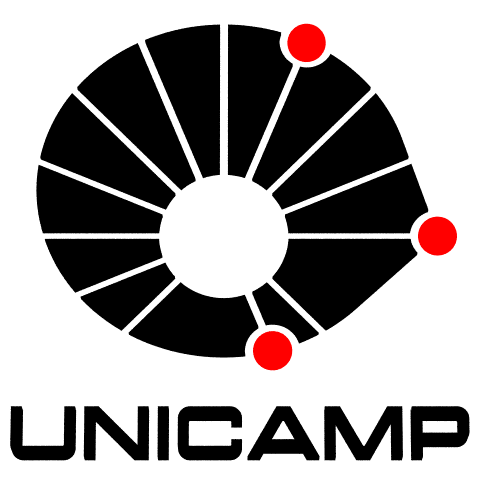
\includegraphics[scale=0.18]{image/LogoUnicamp}
\end{figure} 
%
\vspace*{10pt}
%\text{ }\\[7 cm]
\textbf{\LARGE Exercício de Fixação de Conceitos 2} \\ \vspace{12pt}
\textbf{\large EA072 - Inteligência Artificial em Aplicações Industriais}
\vspace*{72pt}

Gustavo \textbf{CIOTTO PINTON} - \textbf{RA 117136}
 

Campinas, \today

\end{center}
\end{titlepage}

\newpage
%  
% {\large 
%     \centerline{\textbf{Exercício de Fixação de Conceitos 1}}
%     \centerline{Gustavo Ciotto Pinton - 117136}
%     \centerline{EA072 - Inteligência Artificial em Aplicações Industriais}
% }
\section {Introdução}

O principal propósito deste primeiro experimento foi explorar as ferramentas
disponibilizadas pelo \textit{software} \textit{Code Warrior}, uma interface
gráfica baseada na \textit{IDE Eclipse}, para o desenvolvimento de
\textit{firmwares} compatíveis com microcontrolador \textit{Freescale KL25}.
Sendo assim, utilizamos tal plataforma para configurar alguns pinos do
microcontrolador como entrada ou saída, dependendo da montagem desejada. Foram
realizadas, no total, três montagens distintas.

\vspace{12pt}

Na primeira, o objetivo foi construir um programa capaz de piscar o \textit{LED}
vermelho, presente no \textit{kit}, em uma frequência de 1Hz. Para tal, foi
necessário consultar os manuais do microcontrolador [\ref{bib:manual}] para
entender como a comunicação entre ele e o diodo poderia ser realizada e como gerar interrupções
em instantes periódicos de tempo. Em seguida, levando em conta que o
\textit{kit} possui ainda outros dois \textit{LEDs}, extendemos o programa para piscar
também o \textit{LED} verde, a uma frequência de 2Hz.

\vspace{12pt}

A segunda tarefa consistiu na introdução de um \textit{LED} externo, de
modelo \textit{TLDR490} fabricado pela empresa \textit{Vishay} e cuja
documentação é disponibilizada no site do curso [\ref{bib:led}]. Para
realizá-la, foi preciso escolher um pino disponível do microcontrolador para funcionar como
\textit{output} e calcular a resistência necessária para limitar a corrente a
fim de não danificar nenhum dos dois componentes.

\vspace{12pt}

Enfim, a última tarefa envolveu o uso de um \textit{push-button} para fornecer
ao usuário a possibilidade de controlar o funcionamento dos \textit{LEDs}. Para
isso, tivemos de configurar um pino como entrada, assim como escolher
uma resistência para limitar a corrente que passa pelo circuito. Essa
resistência é chamada de \textit{pull} em referência à função que desempenha:
pode induzir um estado padrão alto (\textit{pull up}) ou baixo (\textit{pull
down}) na saída do circuito, que, nosso caso, é o pino que foi configurado como
\textit{input}.

\vspace{12pt}

As próximas seções visam a análise dessas montagens. 

\section {Análise}

Esta seção é dedicada às características que determinam as três montagens.

\subsection{Criação do Projeto} 


\section* {Referências bibliográficas}
\begin {itemize}
  \item \url{https://en.wikipedia.org/wiki/Sunspot}. Acessado às 19:22 29/09/2015.
  \item Guyon, I.; Elisseeff, A. "An introduction to variable and feature selection", Journal of Machine Learning Resear ch, vol. 3, pp. 1157 - 1182 2003.
  \item \url{http://archive.ics.uci.edu/ml/datasets/Wine+Quality}.\\
  	 Acessado às 21:27 30/09/2015.
\end{itemize}

    
\end{document}
